\documentclass{article}
% if you need to pass options to natbib, use, e.g.:
%     \PassOptionsToPackage{numbers, compress}{natbib}
% before loading neurips_2023
\usepackage[final]{neurips}
% to avoid loading the natbib package, add option nonatbib:
%    \usepackage[nonatbib]{neurips}


\usepackage[utf8]{inputenc} % allow utf-8 input
\usepackage[T1]{fontenc}    % use 8-bit T1 fonts
\usepackage{hyperref}       % hyperlinks
\usepackage{url}            % simple URL typesetting
\usepackage{booktabs}       % professional-quality tables
\usepackage{amsfonts}       % blackboard math symbols
\usepackage{nicefrac}       % compact symbols for 1/2, etc.
\usepackage{microtype}      % microtypography
\usepackage{xcolor}         % colors
\usepackage{amsmath}        % math environments
\usepackage{graphicx}       % figures
\usepackage{subcaption}     % subfigures


\title{Automatic Speech Recognition (ASR)}


% The \author macro works with any number of authors. There are two commands
% used to separate the names and addresses of multiple authors: \And and \AND.
%
% Using \And between authors leaves it to LaTeX to determine where to break the
% lines. Using \AND forces a line break at that point. So, if LaTeX puts 3 of 4
% authors names on the first line, and the last on the second line, try using
% \AND instead of \And before the third author name.


\author{%
  Jiarong Edwin Chen\\
  Department of Electrical \& Computer Engineering\\
  University of Toronto\\
  \texttt{edwinece.chen@mail.utoronto.ca} \\
  \And
  Trung-Lam Nguyen\\
  Department of Electrical \& Computer Engineering\\
  University of Toronto\\
  \texttt{trunglam.nguyen@mail.utoronto.ca} \\
  \And
  Anubhav Sharma\\
  Department of Electrical \& Computer Engineering\\
  University of Toronto\\
  \texttt{anubhav.sharma@mail.utoronto.ca} \\
}

\begin{document}


\maketitle


\begin{abstract}
We design and evaluate an end-to-end Automatic Speech Recognition (ASR) system that converts speech to text on the LJSpeech dataset~\cite{ljspeech17}. Starting from a DeepSpeech2-inspired~\cite{amodei2016deep} baseline using unidirectional Gated Recurrent Units (GRUs) with lookahead convolution, we investigate the impact of using different temporal encoders: bidirectional vs.\ unidirectional GRUs, Long Short-Term Memory (LSTM), and Conformer. All models are trained end-to-end using Connectionist Temporal Classification (CTC) loss and evaluated via Character Error Rate (CER) and Word Error Rate (WER). 

\textbf{TODO: one-sentence summary of key finding (e.g., best model, CER value).}
\end{abstract}

\section*{Attestation of Teamwork}
\textbf{TODO: Finalise contributions with all teammates before submission.}
\begin{itemize}
    \item \textbf{Jiarong Edwin Chen}: Research and implementation of baseline Deep Speech 2 and Conformer architecture.
    \item \textbf{Trung-Lam Nguyen}: CNN implementation, data loader optimization, model training and benchmarking.
    \item \textbf{Anubhav Sharma}: Dataset curation, preprocessing, LSTM implementation, model performance and training optimization.
\end{itemize}

\section{Introduction}
Automatic Speech Recognition (ASR) is a foundational problem in deep learning with wide-ranging real-world impact. In education, for example, accurate lecture transcription can reduce cognitive load, improve review efficiency, and enable new modes of interaction with learning material~\cite{grandview2025speech}.

The goal of this project is to build a performant ASR system that converts speech to text. This task is inherently difficult due to the high-dimensional nature of acoustic signals, variations in speaking rates and accents, and complex temporal dependencies between spoken sounds~\cite{zambreno2025evaluating}.

Traditional ASR pipelines relied on hand-crafted acoustic models, pronunciation dictionaries, and Hidden Markov Models, requiring substantial expert linguistic knowledge~\cite{juang2005automatic}. Deep learning architectures can instead learn robust representations from diverse speech data without such expertise. End-to-end (E2E) models — such as the DeepSpeech2 variant implemented here — unify the acoustic, pronunciation, and language modelling components into a single trainable architecture, significantly simplifying the overall pipeline~\cite{amodei2016deep}.

\section{Problem Formulation and Preliminaries}
\label{sec:prelim}

\subsection{Problem Statement}

ASR is the task of mapping a continuous acoustic input to a discrete textual transcription. Given a variable-length sequence $X = (x_1, x_2, \ldots, x_T)$ where the frame $x_t \in \mathbb{R}^F$ represents $F$-dimensional spectral features at time step $t$, the goal is to learn a mapping $f_\theta: \mathbb{R}^{T \times F} \to \mathcal{V}$ that produces the target sequence $y = (y_1, \ldots, y_L)$ over vocabulary $\mathcal{V}$. We use the character-level vocabulary of the \texttt{facebook/wav2vec2-base} CTC tokenizer~\cite{wolf-etal-2020-transformers}. The training objective is to minimise CER and WER over held-out audio.

\subsection{Mel Spectrogram}

Raw audio waveforms are high-dimensional and contain information redundant to transcription. We transform each waveform into a Mel spectrogram to produce a compact representation. The Short-Time Fourier Transform (STFT) first partitions the signal into overlapping windows of $n_\text{fft} = 512$ samples with hop length $H = 256$ samples, and computes a Discrete Fourier Transform on each window to obtain a time-frequency spectrogram. A bank of $F = 80$ triangular Mel filters then re-maps the linear frequency axis to the Mel scale, which approximates the logarithmic sensitivity of human hearing~\cite{mel_scale_rationale}. The resulting matrix $X \in \mathbb{R}^{T \times 80}$ is the direct model input, with a sample rate of 16\,kHz.

\textbf{TODO: CONSIDER LEAVING IN BECAUSE TAUGHT IN CLASS ALREADY}
\subsection{Connectionist Temporal Classification (CTC)}

A key challenge in ASR is that the target transcript length $L$ is typically far shorter than the input sequence length $T$, and frame-level alignment labels are unavailable.

CTC~\cite{graves2006connectionist} resolves this by introducing a \textit{blank} token $\epsilon$ and defining $\mathcal{B}^{-1}(y)$ as the set of all length-$T$ \textit{paths} $\pi$ — sequences of characters (including blanks and repetitions) that collapse to the target sequence $y$ after merging consecutive repeated characters and removing blanks. The CTC loss is the negative log-likelihood of $y$ marginalised over all valid paths:
\begin{equation}
    \mathcal{L}_\text{CTC} = -\log \sum_{\pi \,\in\, \mathcal{B}^{-1}(y)} \prod_{t=1}^{T} p(\pi_t \mid X).
    \label{eq:ctc}
\end{equation}
This allows the model to be trained end-to-end without manual alignment annotation. At inference time, we apply greedy decoding: the highest-probability character is selected at each time step and the resulting path is collapsed to produce the final transcript.

\subsection{Evaluation Metrics}

Performance is assessed using two standard edit-distance-based metrics:
\begin{equation}
    \text{CER} = \frac{S_c + D_c + I_c}{N_c}, \qquad \text{WER} = \frac{S_w + D_w + I_w}{N_w},
\end{equation}
where $S$, $D$, and $I$ denote substitutions, deletions, and insertions, and $N$ is the total reference length in characters ($N_c$) or words ($N_w$). CER is the primary metric for this work, as it is more granular and better aligned with a character-level output model; WER is reported for completeness.

\subsection{Language-Model-Augmented Decoding with KenLM}

Greedy CTC decoding constructs the output sequence by selecting the most probable character at each time step, ignoring linguistic context and frequently producing implausible character sequences.

CTC beam search maintains the top-$k$ partial hypotheses at each step, allowing it to consider the overall likelihood of the partial sequences instead. However, without a language model, beam search does not provide significant improvements as there is no linguistic information to influence the hypotheses.

KenLM~\cite{heafield-2011-kenlm} is an efficient $n$-gram language model that assigns a log-probability to any word sequence based on corpus statistics. Rescoring with KenLM combines the acoustic and language model scores for each beam hypothesis $h$:
\begin{equation}
    \text{score}(h) = \log p_\text{acoustic}(h) + \lambda \log p_\text{LM}(h) + \beta \cdot |h|_w,
    \label{eq:lm_decode}
\end{equation}
where $\lambda$ (LM weight) controls the influence of the language model, $\beta$ (word score) is a per-word bonus that encourages or penalises longer transcriptions, and $|h|_w$ is the number of words in $h$. The beam is pruned to the top-$k$ hypotheses after each step. This requires only a pre-trained ARPA-format $n$-gram model and a pronunciation lexicon --- no retraining of the acoustic model. In our implementation we use a 3-gram KenLM model with $\lambda = 1.5$ and $\beta = -0.5$.

\subsection{Variable-Length Inputs and Packed Padding}

Audio recordings within a mini-batch differ in duration. Padding shorter sequences to match the longest enables batch-parallel processing, but passing these padded sequences through an RNN corrupts hidden states as each pad step accumulates activations that are independent of the actual speech content, causing gradients to incorrectly attribute error to real frames. PyTorch's \texttt{pack\_padded\_sequence} and \texttt{pad\_packed\_sequence} utilities~\cite{paszke2019pytorch} address this by packing only real (non-pad) frames into the RNN computation graph, so that the recurrent update and gradient flow bypass padding tokens entirely.

\section{Design}

\subsection{Dataset: LJ Speech}

We train and evaluate all models on the LJ Speech dataset~\cite{ljspeech17}, which comprises 13,100 transcribed short audio clips of a single speaker with an average duration of approximately 7 seconds. Its clean, single-speaker recordings provide low variability in pronunciation and recording conditions, making it an effective sandbox for iterating on architecture with limited compute~\cite{mou2024performance}. Audio is resampled to 16\,kHz and transcriptions are upper-cased to match the CTC tokenizer vocabulary~\cite{wolf-etal-2020-transformers}; characters outside the tokenizer vocabulary are removed.

\subsection{Architecture}

Our baseline model follows the DeepSpeech2 architecture~\cite{amodei2016deep} but scaled to train on the smaller LJ Speech dataset and limited compute. We then adapted the baseline to explore different temporal encoders, as shown in Figure~\ref{fig:architecture}.

\begin{figure}[h]
    \centering
    % 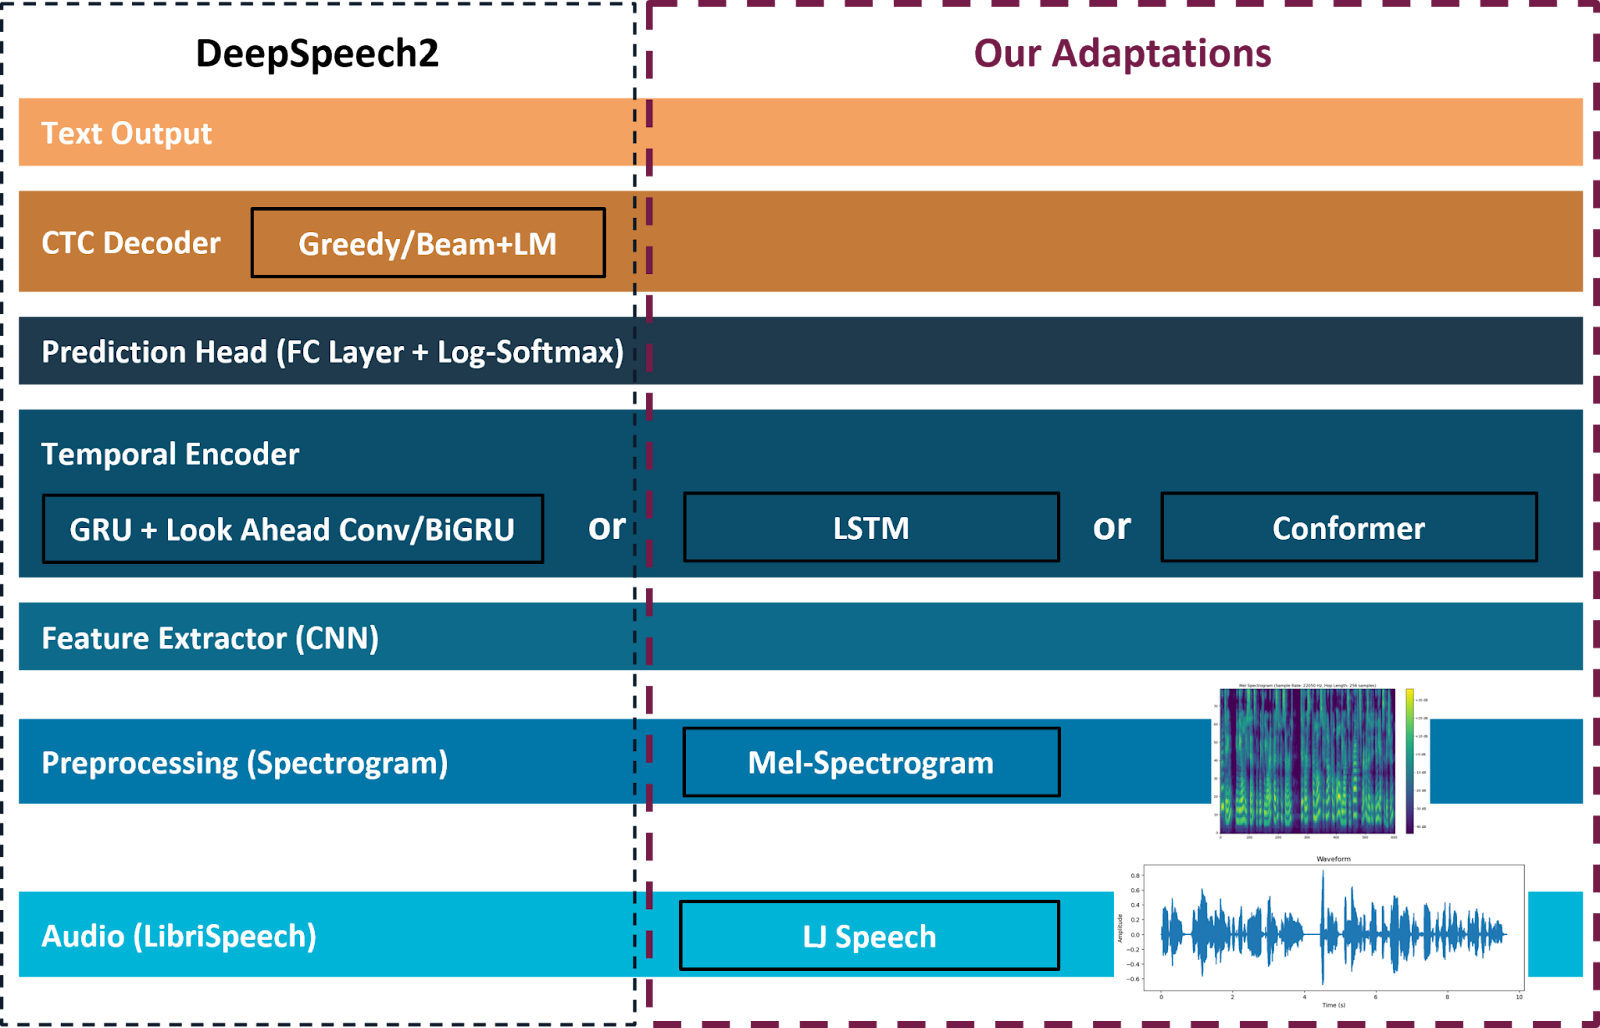
\includegraphics[width=0.88\linewidth]{model.png}
    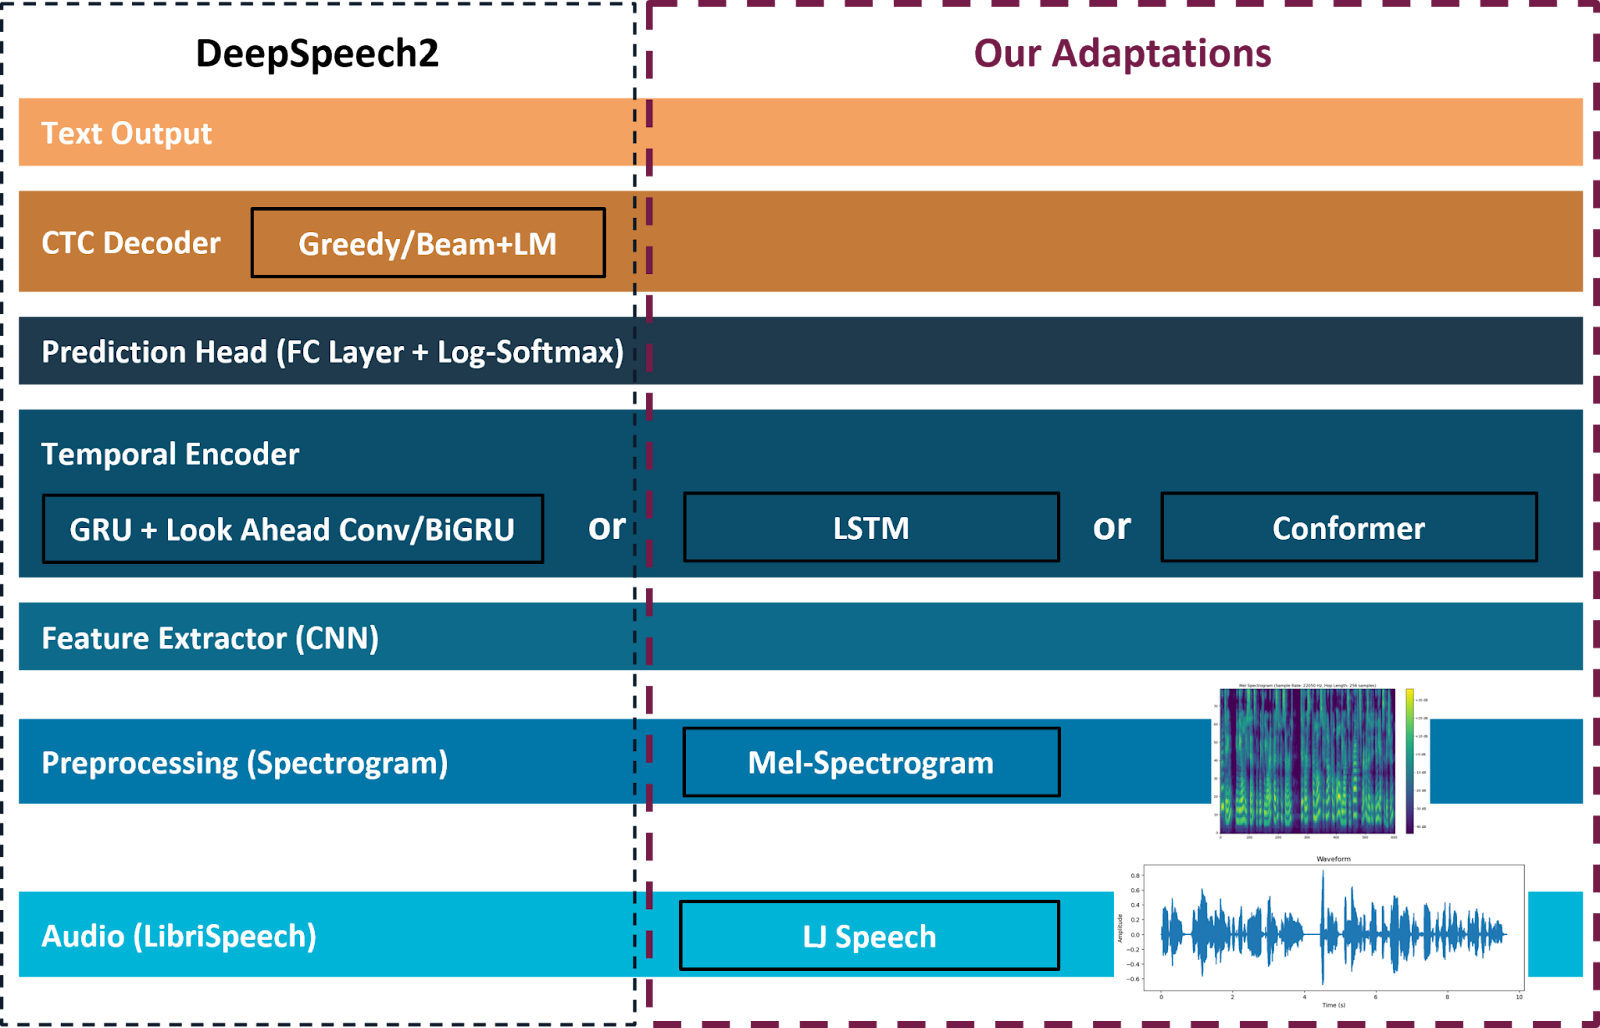
\includegraphics[scale=0.18]{model.png}
    \caption{Baseline model based on the DeepSpeech2 architecture and our adapted models}
    \label{fig:architecture}
\end{figure}

\textbf{Preprocessing.}
Raw audio data is first converted to Mel-spectrograms, distilling information relevant to transcription.

\textbf{Feature Extractor.}
A 2D Convolutional network extracts time-frequency features by learning local structures in the input Mel-spectrograms. This also reduces channel dimensionality, compressing the time-frequency information into smaller, more informative feature spaces.

\textbf{Temporal Encoder.}
Encodes the time-sequential relations across the features in a time-sequence of hidden states. Here we experiment with the GRU, LSTM, and Conformer ~\cite{gulati2020conformer} encoders, as well as different configurations for each of the encoders and compare their trade-offs.

\textbf{Prediction Head.}
Final linear layer that maps the hidden states to token log-probabilities. Log-probabilities are used instead of probabilities to improve numerical stability when computing the CTC loss.

\textbf{CTC Decoder.}
Computes the CTC loss during training and outputs the predicted character sequence during inference.





% \section{Methodology}
% TODO: Fill in training details (optimizer, LR schedule, batch size, epochs, gradient clipping).
% TODO: Describe multi-seed evaluation protocol (seeds: 1508, 2603, 9102).
% TODO: Describe CTC greedy decoding and any LM-augmented beam search used.
\section{Methodology}

%------------------------------------------------------------------
\subsection{Implementation Stack}
%------------------------------------------------------------------

Models are implemented in PyTorch~\cite{paszke2019pytorch}, with \texttt{torchaudio}~\cite{hwang2023torchaudio}
for audio processing and CTC beam-search decoding. The character vocabulary is provided by the
\texttt{facebook/wav2vec2-base} tokenizer via Hugging Face \texttt{transformers}~\cite{wolf-etal-2020-transformers}.
CER and WER are computed using \texttt{torchmetrics}~\cite{Detlefsen2022}.

%------------------------------------------------------------------
\subsection{Shared CNN Feature Extractor}
\label{sec:cnn}
%------------------------------------------------------------------

All model variants share a two-layer 2-D convolutional front-end
(\(\text{Conv2D} \to \text{BatchNorm2D} \to \text{Clipped ReLU}\), where
\(\sigma(x) = \min(\max(x,0),20)\)), clipping activations at 20 to prevent exploding
values that can destabilise CTC training.
The first layer uses a \(41\times11\) kernel with stride \(2\times2\) and padding \(20\times5\);
the second uses a \(21\times11\) kernel with stride \(2\times1\) and padding \(10\times5\)
(frequency\(\times\)time).

%------------------------------------------------------------------
\subsection{Temporal Encoder Variants}
%------------------------------------------------------------------

\subsubsection{GRU / LSTM}

Both the GRU and LSTM use gated recurrent units to mitigate vanishing gradients; the LSTM additionally maintains an explicit cell state for stronger long-range memory.
Both variants use \(L=3\) stacked layers with hidden size 512, LayerNorm between layers, and dropout \(p=0.3\).
We evaluate unidirectional and bidirectional GRU; the unidirectional variant is followed by an additional \emph{look-ahead convolution} (kernel size 41, right-padded) for bounded future context.

\subsubsection{Conformer}

The Conformer~\cite{gulati2020conformer} augments a multi-head self-attention (MHSA) transformer
with a depthwise convolutional module interleaved between each attention layer.
Self-attention captures global dependencies across the full sequence in parallel,
while the convolution module provides a local-pattern inductive bias that pure transformers lack.
The \(\mathcal{O}(n^2)\) memory cost of self-attention is acceptable for the utterance lengths
in LJ Speech.
We substitute relative positional encoding with absolute sinusoidal encoding, which suffices for this single-speaker corpus and reduces compute.
The shared CNN front-end serves as the convolutional subsampling stage.
We explored 2 Conformer configurations:

\begin{table}[h]
\label{tab:conformers}
  \centering
  \begin{tabular}{lll}
    \toprule
    Latent Dimension & \#Conformer Blocks & \#Parameters (M) \\
    \midrule
    256 & 12 & 18 \\
    144 & 10 & 5 \\
    \bottomrule
  \end{tabular}
\end{table}

and both with 4 self-attention heads, dropout $=0.1$, and depthwise convolution kernel size $=15$.

%------------------------------------------------------------------
\subsection{Training}
%------------------------------------------------------------------

All models are trained end-to-end with Adam + OneCycleLR, mixed-precision (using \texttt{torch.amp}),
and gradient clipping. The best checkpoint is selected by validation WER.

\subsubsection{Replication}

To obtain statistically reliable estimates of model performance and to avoid reporting results that
are artefacts of a particular random initialisation, each model configuration is trained under
three seeds (1508, 2603, and 9102). Before each run, \texttt{torch.manual\_seed}, \texttt{numpy.random.seed},
and Python's built-in \texttt{random.seed} are all set to the chosen seed, allowing our results to be reproducible.
Performance metrics (CER and WER) are reported as the mean \(\pm\) 1 standard deviation across the
three seeds.
This guards against over-stating the benefit of any single architecture choice and enables
fair pairwise comparison between model variants.



\section{Numerical Experiments}
% TODO: Replace all TODO entries with final experimental results.
% TODO: Add learning curve figures (CER, WER, CTC Loss per epoch).

\subsection{Baseline Model Performance}

\begin{table}[h]
  \caption{Baseline model (unidirectional GRU + lookahead convolution) on LJSpeech after convergence.}
  \label{tab:baseline}
  \centering
  \begin{tabular}{lll}
    \toprule
    Model                        & WER     & CER     \\
    \midrule
    Baseline (GRU, unidirectional) & 38.14\% & 12.18\% \\
    \bottomrule
  \end{tabular}
\end{table}

\subsection{Architecture Comparison}

\begin{table}[h]
  \caption{Architecture comparison on the LJSpeech test set. WER/CER reported without LM rescoring
  unless stated. The bidirectional GRU was evaluated over three random seeds (mean $\pm$ std);
  all other entries are single-run results. The rightmost column shows WER after 3-gram KenLM rescoring.}
  \label{tab:comparison}
  \centering
  \begin{tabular}{lllll}
    \toprule
    Architecture                  & CTC Loss & CER        & WER        & WER (LM)   \\
    \midrule
    GRU (uni, 3-layer)            & 0.32     & 11.1\%     & 35.2\%     & 29.8\%     \\
    GRU (uni, 3-layer + lookahead)& 0.31     & 10.7\%     & 33.2\%     & 29.5\%     \\
    GRU (uni, 5-layer)            & 0.27     & 9.9\%      & 29.9\%     & 28.2\%     \\
    GRU (bi, 3-layer)$^\dagger$   & 0.31     & $11.0 \pm 0.10$\% & $33.7 \pm 0.25$\% & 29.2\% \\
    \textbf{LSTM (3-layer)}       & \textbf{0.26} & \textbf{9.2\%} & \textbf{27.7\%} & \textbf{27.8\%} \\
    Conformer (5\,M)              & 0.34     & 11.2\%     & 34.6\%     & 29.7\%     \\
    \textbf{Conformer (18\,M)}    & \textbf{0.29} & \textbf{8.63\%} & \textbf{25.2\%} & \textbf{28.5\%} \\
    \bottomrule
  \end{tabular}
  \smallskip\\
  {\small $^\dagger$ Mean $\pm$ std over seeds 1508, 2603, 9102.}
\end{table}

\subsection{Learning Curves}

\begin{figure}[h]
    \centering
    \begin{subfigure}[b]{0.32\textwidth}
        \centering
        
\includegraphics[width=\linewidth]{Report/results/train_cer.png}
        \caption{Train CER}
    \end{subfigure}
    \begin{subfigure}[b]{0.32\textwidth}
        \centering
        
\includegraphics[width=\linewidth]{Report/results/train_wer.png}
        \caption{Train WER}
    \end{subfigure}
    \begin{subfigure}[b]{0.32\textwidth}
        \centering
        
\includegraphics[width=\linewidth]{Report/results/train_loss.png}
        \caption{Train Loss}
    \end{subfigure}
    \caption{Training metrics for all model variants.}
    \label{fig:learning_curves}
\end{figure}

\section{Discussion}

\textbf{Bidirectionality vs.\ lookahead convolution.}
The 3-layer bidirectional GRU (33.7\% WER, 11.0\% CER) does not improve over the lookahead convolution baseline (33.2\% WER, 10.7\% CER), despite having access to full future context. This suggests that a fixed-width look-ahead window is sufficient for a low-variability, single-speaker corpus, and full bidirectionality adds parameter cost without proportionate accuracy gain. The multi-seed standard deviation for the bidirectional GRU ($\pm 0.25\%$ WER, $\pm 0.10\%$ CER) is small, indicating stable convergence across random seeds.

\textbf{GRU vs.\ LSTM.}
The 3-layer LSTM (27.7\% WER, 9.2\% CER) outperforms all 3-layer GRU variants on greedy-decoded WER. With LM rescoring the gap narrows (LSTM: 27.8\% vs.\ bidirectional GRU: 29.2\%), and a 5-layer GRU (29.9\% WER) partially recovers it, suggesting that GRU gating capacity at 3 layers is the bottleneck rather than the gating mechanism itself.

\textbf{Conformer encoder.}
The 18\,M-parameter Conformer achieves the best greedy WER (25.2\%) and CER (8.63\%), outperforming all recurrent variants. Interestingly, LM rescoring raises its WER to 28.5\%, suggesting its character-level distributions are already more linguistically plausible. The 5\,M Conformer underperforms all recurrent models, highlighting the critical role of model capacity for self-attention.

\textbf{LM rescoring.}
KenLM beam-search rescoring reduces WER for every architecture except the LSTM and Conformer. Gains are largest for the weakest acoustic models (uni-GRU: $35.2\% \to 29.8\%$, $-5.4$\,pp) and negligible for stronger ones (LSTM: $27.7\% \to 27.8\%$), consistent with the LM filling gaps left by a weaker acoustic signal.


\section{Conclusions}

Among four end-to-end ASR architectures evaluated on LJSpeech, the 18\,M-parameter Conformer achieved the best performance, while the LSTM outperformed all GRU variants at the same depth. Contrary to expectations, full bidirectionality offered no gain over the lookahead convolution baseline, suggesting limited future context suffices for a clean, single-speaker corpus. KenLM rescoring helped weaker models but was largely redundant for stronger ones. Future work could explore diverse datasets such as LibriSpeech, pre-trained features from wav2vec 2.0, and SortaGrad curriculum training.


\bibliographystyle{unsrt}
\bibliography{ref.bib}

\section*{Appendix}
Any descriptions about supplementary materials go here.


\newpage
\section*{Use of AI}
AI assistants (GitHub Copilot and Claude) were used as coding aids throughout this project, specifically to: generate boilerplate code for data loading and training pipelines, suggest debugging strategies for shape mismatches in RNN/CTC pipelines, and assist in drafting report text. All AI-generated outputs were reviewed, verified, and edited by team members. AI was not used to run experiments or generate results.
% TODO: Revise to accurately reflect the team's actual AI usage before submission.

\section*{Consent for Information Sharing}
As part of this course, we may share selected project materials (e.g., reports, presentation slides, and presentation recordings) on the course webpage as learning resources for future students. Additionally, we may use anonymized project information for internal statistical analysis of course outcomes. Please indicate your preferences below. \textit{Your choices will not affect your grade in any way.}

\subsection*{Consent for Sharing Project Materials}
\textit{Please keep the item you wish and remove the other one.}

\begin{itemize}
	\item All group members consent to allow the project materials (report, slides, and presentation recording) to be shared on the course page for future students.
	\item The group members do \textbf{not} consent to allow the project materials (report, slides, and presentation recording) to be shared on the course page for future students.
\end{itemize}



\subsection*{Consent for Use of Project Information in Statistical Analysis}
\textit{Please keep the item you wish and remove the other one.}
\begin{itemize}
	\item All group members consent to allow anonymized information about the project (e.g., topic, methods, outcomes, grades) to be used by the instructor for statistical analysis and course improvement.
	\item The group members do \textbf{not} consent to allow anonymized information about the project (e.g., topic, methods, outcomes, grades) to be used by the instructor for statistical analysis and course improvement.
\end{itemize}

\subsection*{Optional Comments}
\textit{Please list any specific conditions or comments here.}

\subsection*{Group Identification}

\begin{itemize}
	\item Group number: 8
	\item Names of group members: Jiarong Edwin Chen, Trung-Lam Nguyen, Anubhav Sharma
	\item Signature of group members:
	\item Date:
\end{itemize}

\end{document}
